 \newchapter{feedforward}{Feedforward Results}

This is the introductory text.

\newsection{gainScans}{Gain Scans}


\newsection{jitterRecord}{Lowest Achieved Phase Jitter}

The results presented in this section show the best downstream phase jitter currently achieved at CTF3 with the PFF correction. The dataset was taken on Friday 20th November 2015 at 15:38 as one of a sequence of short measurements fine-tuning the gain around the optimal value. Results from the other datasets in this sequence are discussed in the following section to demonstrate the phase stability achieved a longer time scales. The 15:38 dataset shown here comprises 150 pulses taken in interleaved mode, with the correction applied to the 75 odd indexed pulses and no correction applied to the remaining 75 even indexed pulses. The used gain in FONT5a units was 800, corresponding to a real applied correction of 1.13 times the upstream phase using the conversion factor calculated in \ref{ss:fontSetup}.

Naturally, this dataset was taken during the best beam conditions currently achieved at CTF3 in terms of phase propagation, taken just after a series of R56 and beam energy optimisations using the same methods discussed in Chapter \ref{c:phasePropagation}.

\begin{table}
  \begin{center}
    \begin{tabular}{| c | c | c | c |}
	   \hline
       Correction Status & Upstream Jitter & Downstream Jitter & Correlation \\ \hline
       FF Off & \(0.69\pm0.06^\circ\) & \(0.74\pm0.06^\circ\) & \(0.93\pm0.04\) \\
	   FF On & \(0.57\pm0.05^\circ\) & \(0.28\pm0.02^\circ\) & \(0.19\pm0.12\) \\
	   FF Simulated & \(0.69\pm0.06^\circ\) & \(0.27\pm0.02^\circ\) & \(0.06\pm0.12\) \\ \hline
    \end{tabular}
    \caption{Best PFF results.}
  	\label{t:BestFF}
  \end{center}
\end{table}

Distribution of points at around 0.5 degrees downstream.

Residual uncorrelated phase (mean and along pulse).

Jitter along pulse

\begin{figure}
  \centering
  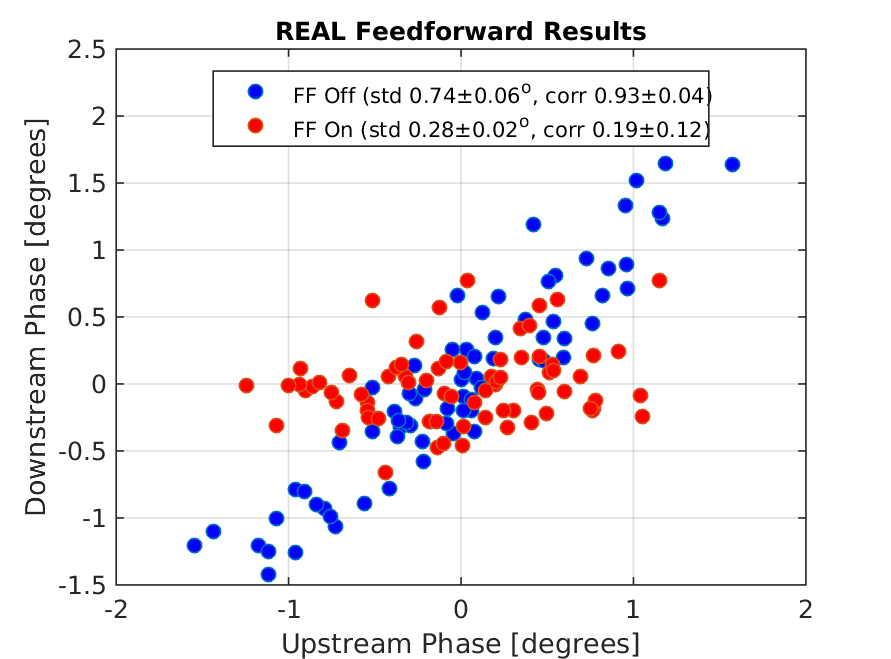
\includegraphics[width=0.45\textwidth]{Figures/feedforward/BestFF_Real}
  \caption{Mean phase.}
  \label{f:BestFF_Real}
\end{figure}

\begin{figure}
  \centering
  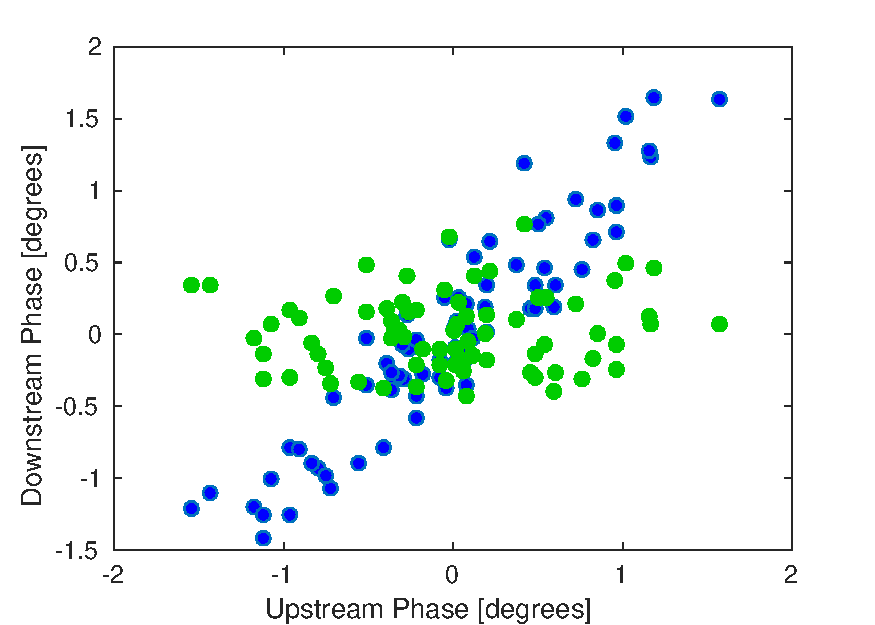
\includegraphics[width=0.45\textwidth]{Figures/feedforward/BestFF_Simulated}
  \caption{Simulated PFF.}
  \label{f:BestFF_Simulated}
\end{figure}


\begin{figure}
  \centering
  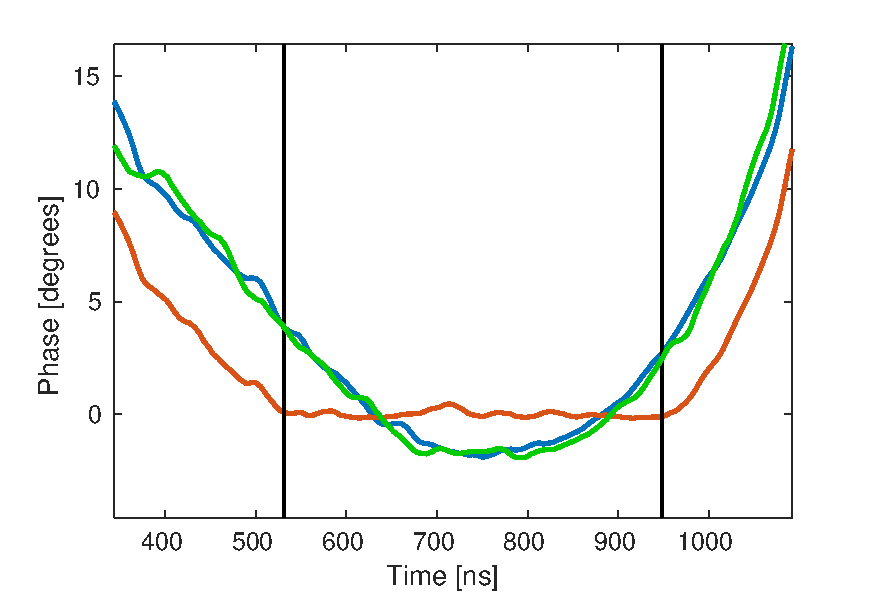
\includegraphics[width=0.45\textwidth]{Figures/feedforward/BestFF_MeanPhaseAlong}
  \caption{Mean phase along.}
  \label{f:BestFF_MeanPhaseAlong}
\end{figure}

\begin{figure}
  \centering
  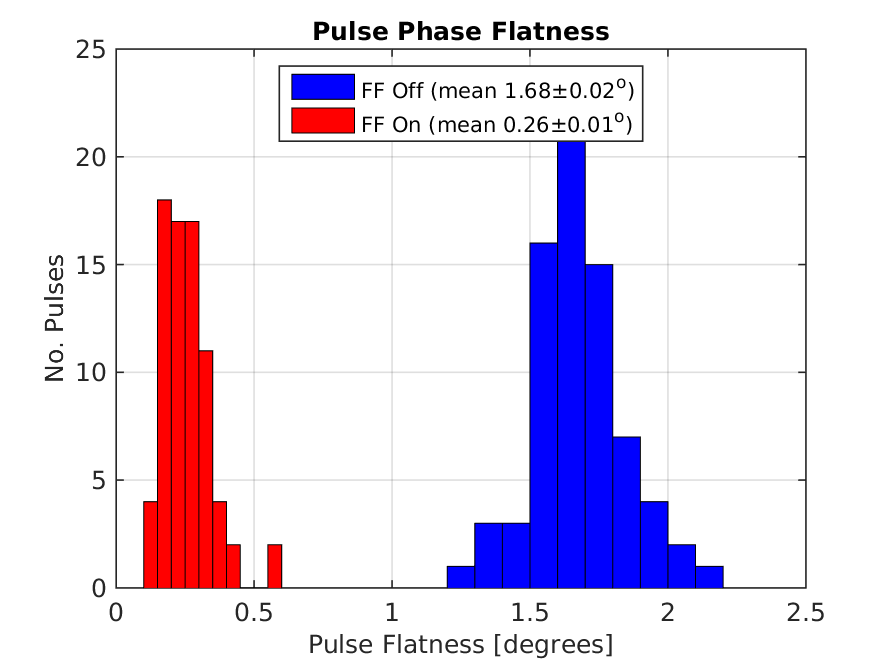
\includegraphics[width=0.45\textwidth]{Figures/feedforward/BestFF_Flatness}
  \caption{Flatness.}
  \label{f:BestFF_Flatness}
\end{figure}

\newsection{longPFF}{Correction on Longer Time Scales}

At CLIC 0.2 degrees phase stability would clearly have to be maintained for much longer time scales than a few minutes. This section therefore discusses the status of the correction across longer time scales, using data from around 15:30 to 18:00 on the 20th November 2015, the same day as the record result previously shown which was taken during this period at 15:38. The PFF system was not operated continuously throughout this two and a half hour window but 15 individual datasets of a few hundred pulses each were taken and these results have been combined to create a large sample of 3083 interleaved pulses (1541 with the correction on and 1542 with the correction off).

\begin{landscape}

\begin{figure}
  \centering
  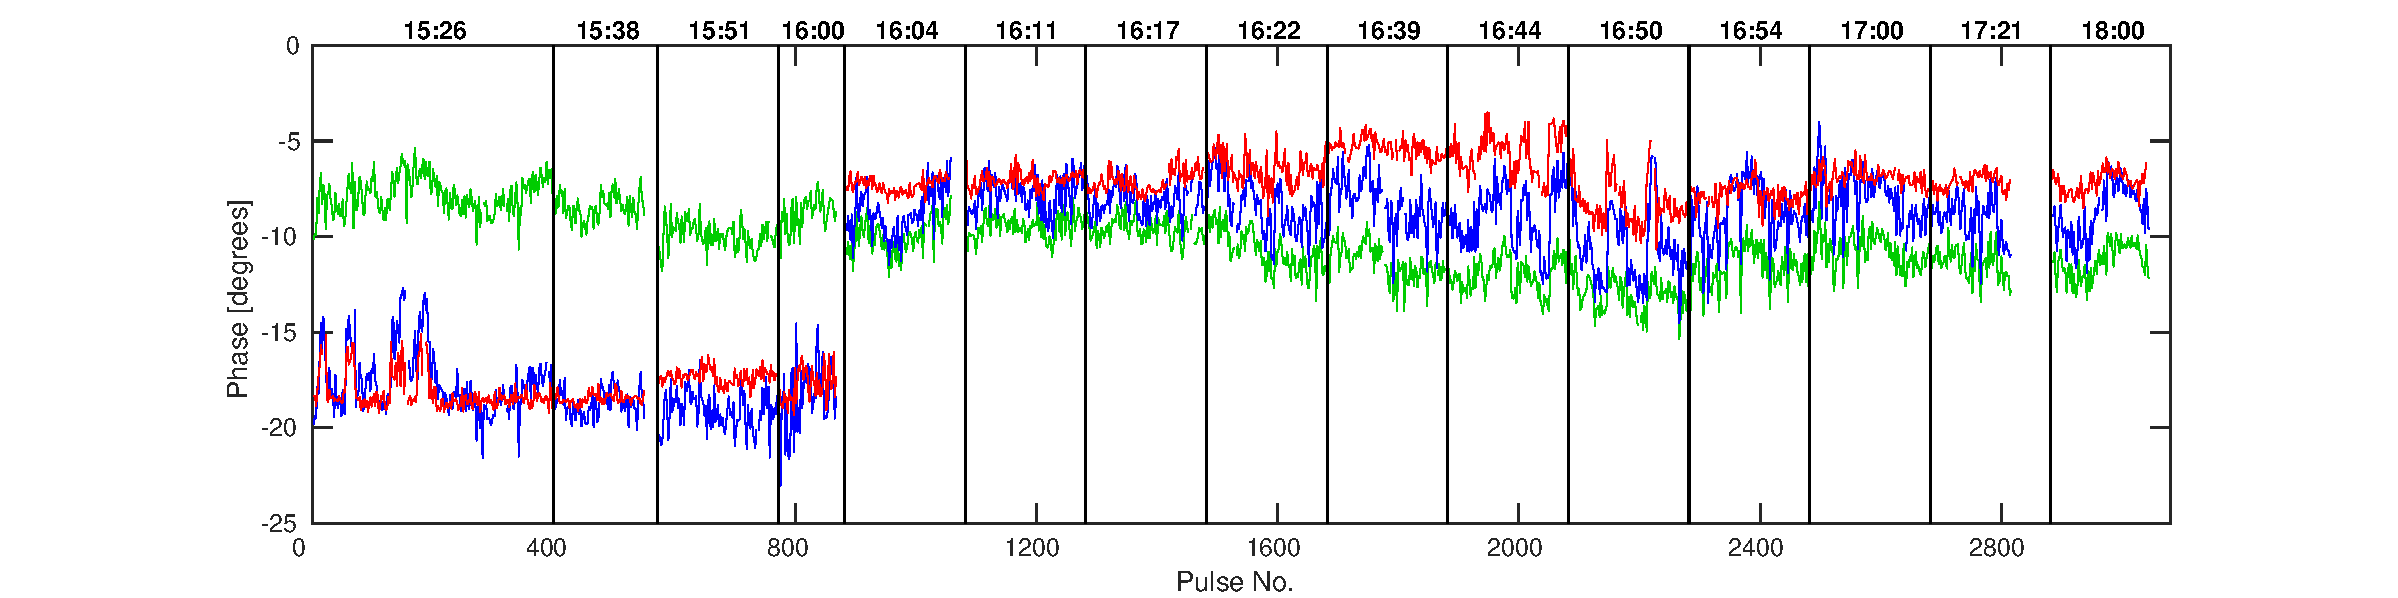
\includegraphics[width=\hsize]{Figures/feedforward/longFF_noMeanSubHistory}
  \caption{History of mean phase across datasets.}
  \label{f:longFF_noMeanSubHistory}
\end{figure}


\begin{figure}
  \centering
  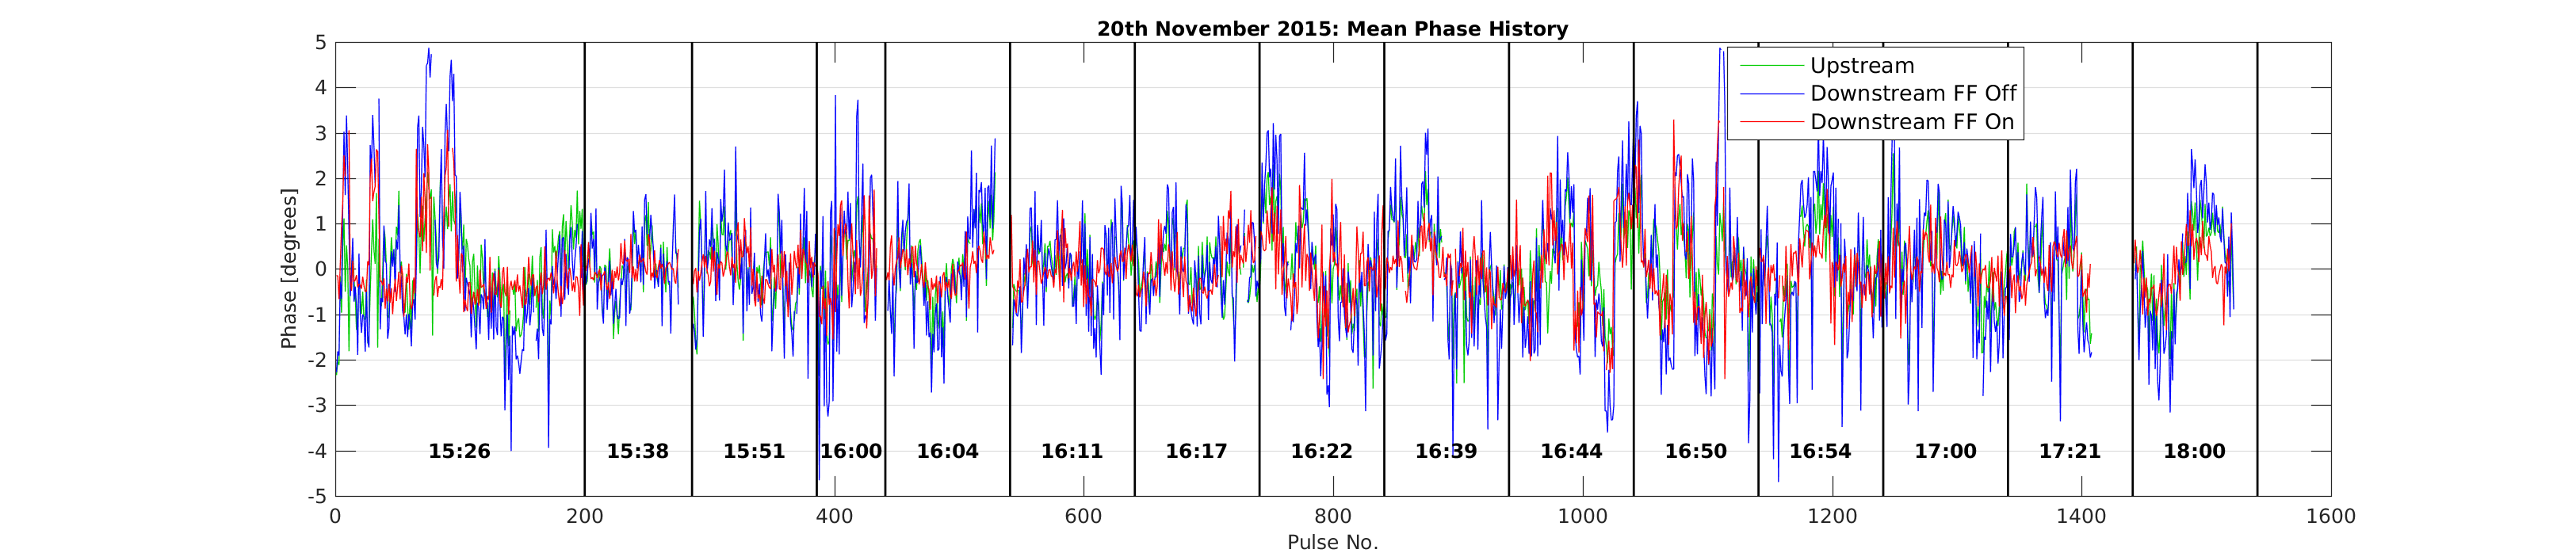
\includegraphics[width=\hsize]{Figures/feedforward/longFF_history}
  \caption{History of mean phase across datasets, with mean subtraction.}
  \label{f:longFF_history}
\end{figure}

\end{landscape}

The raw history of the mean phases upstream and downstream with the correction on and off in the combined data are shown in Figure \ref{f:longFF_noMeanSubHistory}. The time span of each individual dataset is marked by vertical black lines and the times displayed on the plot represent the start time of each dataset. Over the course of the afternoon the mean upstream phase, in green, varies by ten degrees peak-to-peak or \(1.75 \pm 0.02^\circ\) in terms of jitter. Small drifts of up to a few degrees in the upstream phase are not an issue for the performance of the PFF correction providing the correlation between the upstream and downstream phase is not degraded. In some cases upstream phase drifts may lead to a loss in correlation, this could be the case if the source of the drift is a variation in beam energy due to the issues discussed in Chapter \ref{c:phasePropagation}, for example. 

However, larger changes in the upstream phase such as the ten degree fluctuation seen here will impact the PFF performance due to the limited correction range of twelve degrees (\(\pm6^\circ\)) combined with the phase sag along the CTF pulse. 

\begin{eqnarray}
	\Delta\phi(t) = \begin{cases}
	-6^\circ, &  \text{if $g\phi_u \geq+6^\circ$.}\\
	+6^\circ, &  \text{if $g\phi_u\leq-6^\circ$}.\\
	-g\phi_u, &  \text{otherwise.}
	\end{cases}
	\label{e:limCorrection}
\end{eqnarray}



Figure \ref{f:longFF_fractInRange} shows the fraction of pulses for which the optimal correction (upstream phase multiplied by the optimal gain) is within the correction range. In the PFF firmware on the FONT5a board it is possible to add an offset to the ADC output corresponding to the upstream phase. If on the FONT5a board this offset has been set up to zero the apparent measured upstream phase (so that the mean voltage sent to the kickers across the afternoon is zero) the effects of limited correction range are small, as the full \(\pm6^\circ\) range can be used to remove phase jitter rather than any static phase offsets. In this case the ideal correction across a 310~ns portion of the pulse is within the \(\pm6^\circ\) range 96\% of the time.

However, as to date this offset has been set up manually small deviations from the ideal case are possible. Figure \ref{f:longFF_fractInRange} also shows the fraction of pulses within the correction range if there is a static two degree offset in the upstream phase. In this case as many as 39\% of pulses are outside the correction range. To mitigate these effects and to get the largest reduction in jitter possible the centring of the upstream phase in the correction range on the FONT5a board is normally adjusted between datasets. As a consequence of this slow drifts in the upstream phase between datasets are not removed in the corrected downstream phase. 

\begin{figure}
  \centering
  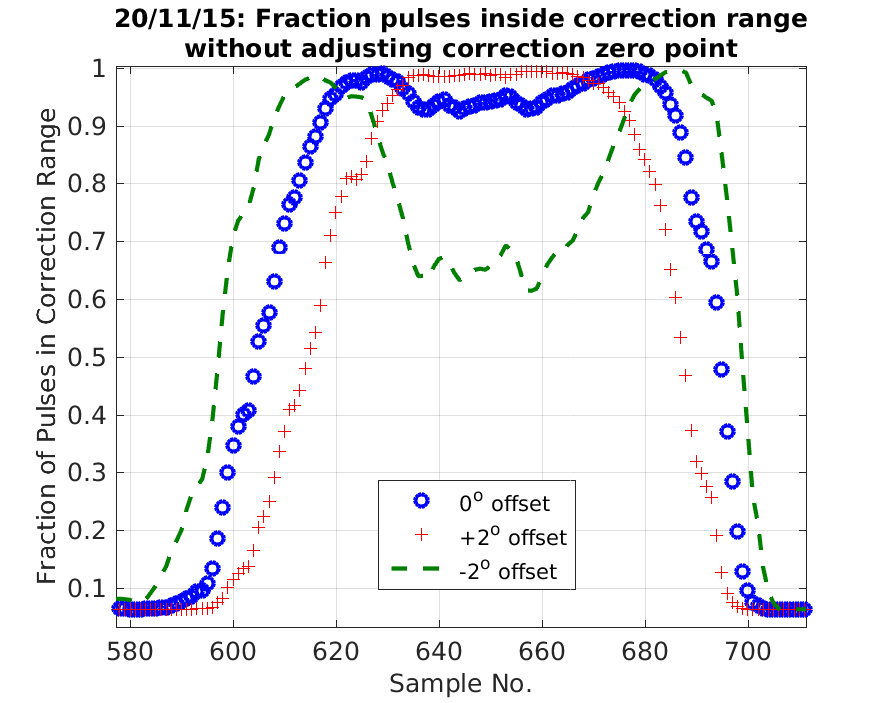
\includegraphics[width=0.45\textwidth]{Figures/feedforward/longFF_fractInRange}
  \caption{Fraction of pulses outside the correction range along the pulse.}
  \label{f:longFF_fractInRange}
\end{figure}


\begin{figure}
  \centering
  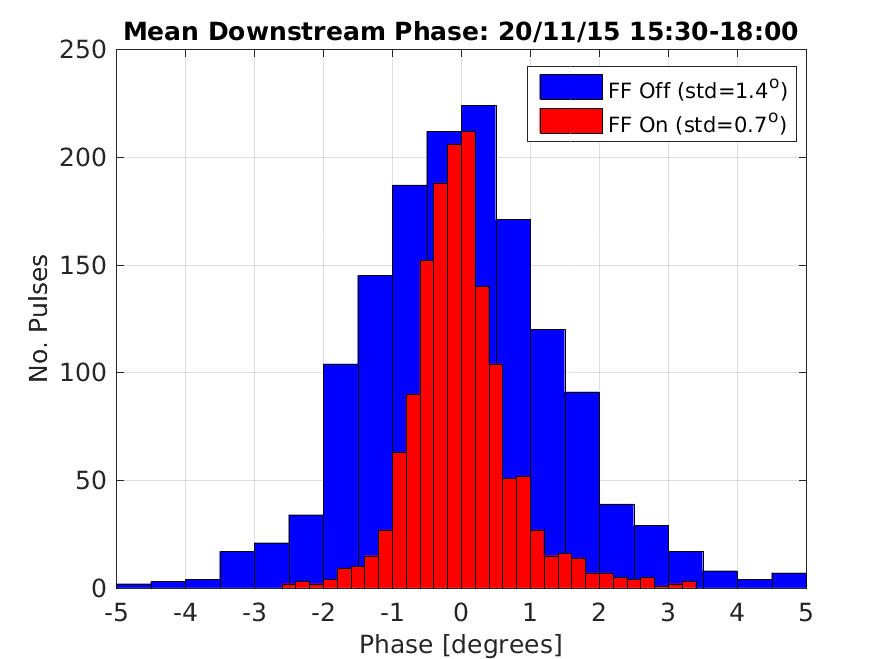
\includegraphics[width=0.45\textwidth]{Figures/feedforward/longFF_histDownstreamPhase}
  \caption{Histogram showing overall distribution of downstream phase with FF off and on.}
  \label{f:longFF_histDownstreamPhase}
\end{figure}

\begin{figure}
  \centering
  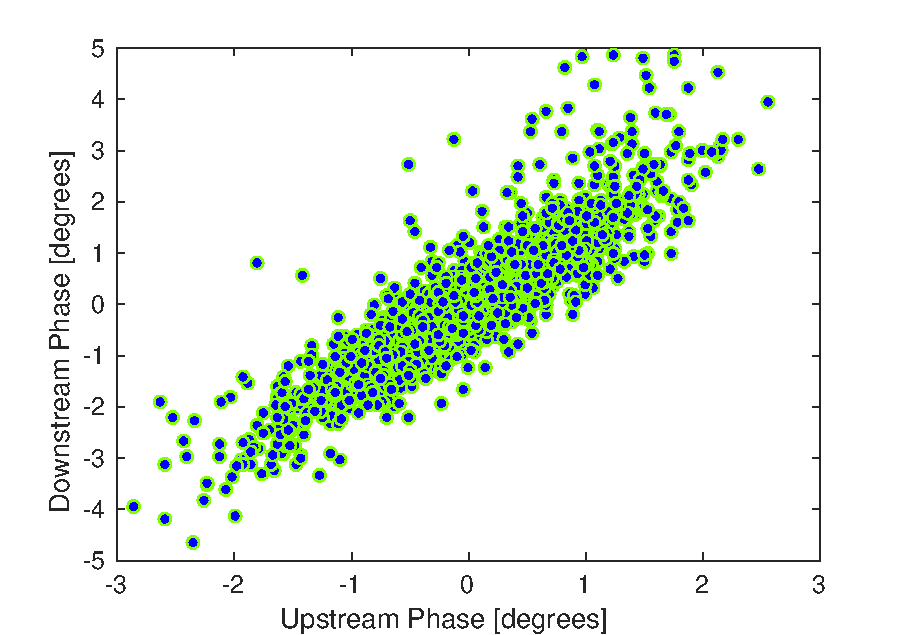
\includegraphics[width=0.45\textwidth]{Figures/feedforward/longFF_scatterFFOff}
  \caption{Downstream phase vs. upstream phase with FF off.}
  \label{f:longFF_scatterFFOff}
\end{figure}

\begin{figure}
  \centering
  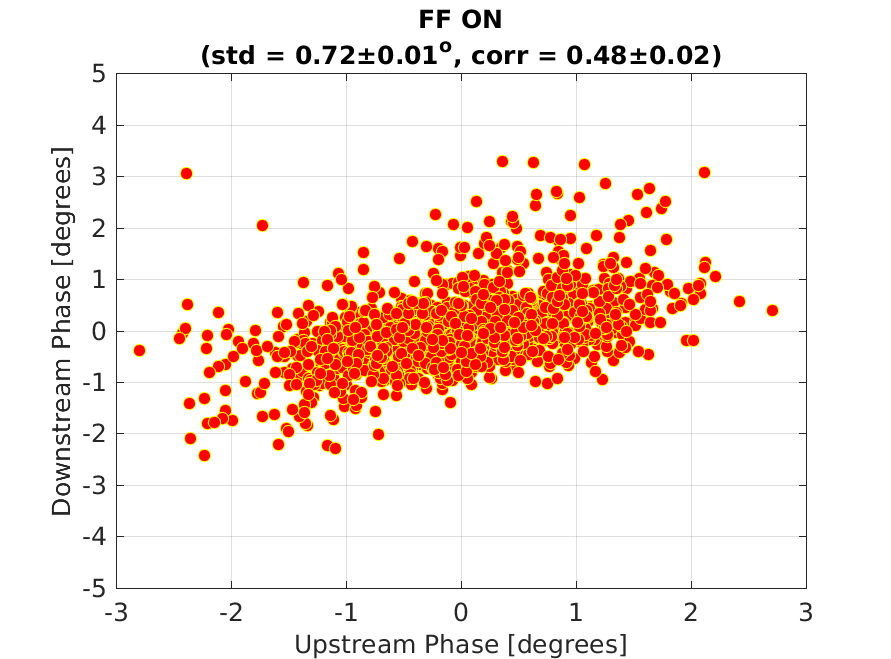
\includegraphics[width=0.45\textwidth]{Figures/feedforward/longFF_scatterFFOn}
  \caption{Downstream phase vs. upstream phase with FF on.}
  \label{f:longFF_scatterFFOn}
\end{figure}

\begin{figure}
  \centering
  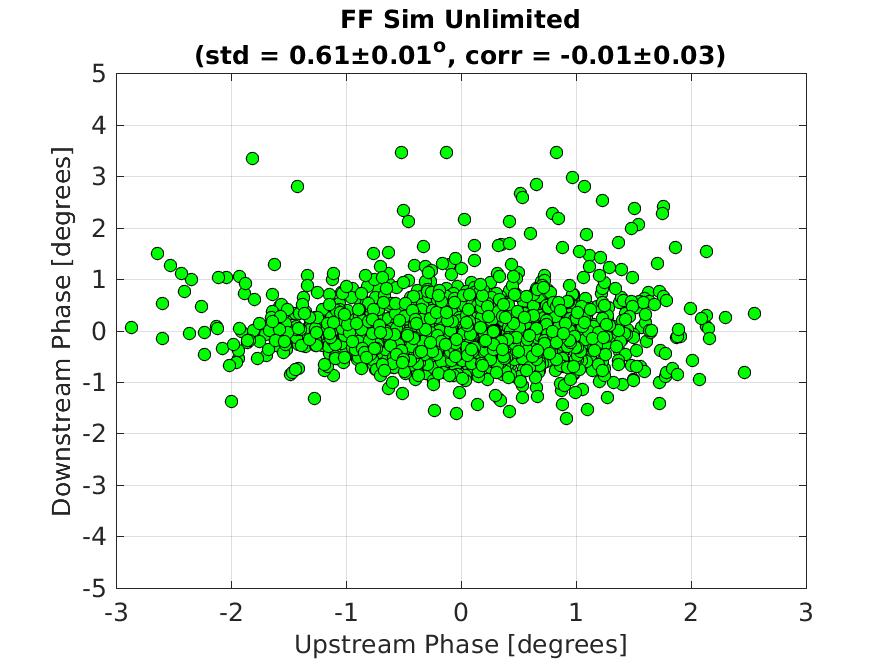
\includegraphics[width=0.45\textwidth]{Figures/feedforward/longFF_scatterFFSimOpt}
  \caption{Downstream phase vs. upstream phase with FF simulated at optimal gain.}
  \label{f:longFF_scatterFFSimOpt}
\end{figure}

\begin{figure}
  \centering
  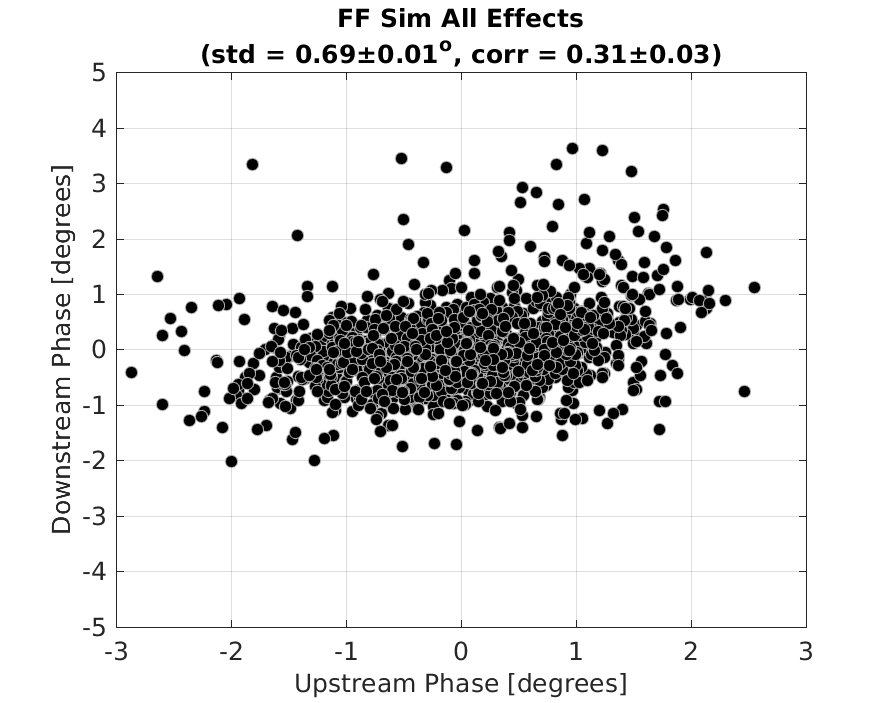
\includegraphics[width=0.45\textwidth]{Figures/feedforward/longFF_scatterFFSimReal}
  \caption{Downstream phase vs. upstream phase with FF simulated with actual gain used.}
  \label{f:longFF_scatterFFSimReal}
\end{figure}

\begin{table}
  \begin{center}
    \begin{tabular}{| c | c | c | c |}
	   \hline
       Correction Status & Upstream Jitter & Downstream Jitter & Correlation \\ \hline
       FF Off & \(0.88\pm0.02^\circ\) & \(1.40\pm0.03^\circ\) & \(0.89\pm0.01\) \\
	   FF On & \(0.86\pm0.02^\circ\) & \(0.72\pm0.01^\circ\) & \(0.48\pm0.02\) \\
	   FF Sim Opt Gain & \(0.88\pm0.02^\circ\) & \(0.61\pm0.01^\circ\) & \(-0.01\pm0.03\) \\
	   FF Sim Real Gain & \(0.88\pm0.02^\circ\) & \(0.68\pm0.01^\circ\) & \(0.35\pm0.02\) \\
	   FF Sim Offset & \(0.88\pm0.02^\circ\) & \(0.69\pm0.01^\circ\) & \(0.36\pm0.02\) \\
	   FF Sim 90\% Real Gain & \(0.88\pm0.02^\circ\) & \(0.72\pm0.01^\circ\) & \(0.46\pm0.02\) \\ \hline
    \end{tabular}
    \caption{Feedforward results using combined data from 20th November 2015.}
  	\label{t:LongFF}
  \end{center}
\end{table}



\newsection{pffNovelSetups}{Correction with Additional Jitter Source}

At CLIC the PFF system will be required to reduce the initial phase jitter by an order of magnitude, from 2 degrees to 0.2 degrees [REF]. With the initial phase jitter of typically 0.8 degrees at CTF3 it is not possible to demonstrate more than a factor 4 reduction in the jitter using the PFF prototype due to hardware limitations, more specifically due to the achieved phase monitor resolution of 0.14 degrees which limits the theoretical best possible correction to 0.2 degrees (Section \ref{s:resolution}). A secondary goal of the PFF prototype in addition to achieving the baseline goal of 0.2 degrees phase jitter is to demonstrate the factor 10 reduction in jitter relevant to CLIC. In order to do this additional sources of phase jitter must be added.

Clearly, the additional source must be prior to the upstream phase monitor in order to add an additional jitter component that is present in both the upstream and downstream monitors. The correlation between the resulting upstream and downstream phase must be  \(99.5\%\) in order for a factor 10 reduction in jitter to be possible (see Section \ref{ss:theoryJitter}). Two different methods to achieve this have been attempted --- firstly by varying the phases of all the klystrons in the injector and secondly by using the non-zero R56 stretching chicane (see Figure \ref{f:ctfLayout}) at the end of the CTF linac in order to intentionally add an energy component to the upstream phase (which propagates downstream).

\newsection{slowCorr}{Slow Correction}

As the PFF system has only a small range of \(\pm6^{o}\), a secondary ``slow phase feedback" or ``slow correction" has also been implemented at CTF3 to be able to remove larger drifts or static offsets in the downstream phase. In principle this slow correction can be used in conjunction with the PFF system to maximise its performance by keeping the mean uncorrected phase well-centred (zeroed) within its \(\pm6^{o}\) range so that the full power of the PFF amplifiers can be used to correct the fast pulse-to-pulse and intra-pulse phase jitter. If the beam phase were to drift away by \(15^{o}\), for example, the calculated PFF correction would saturate the amplifier across the full pulse length to give the maximal shift of \(6^{o}\). In this case the drift would be partially removed downstream but the PFF system would no longer have any effect on the phase jitter (as the output voltage to the kickers is constant in saturation rather than varying with the phase).

The design and results from the slow correction are discussed in this section. To date its main use has been to verify the ability to shift the beam phase in the TL2 chicane in early-2014 prior to the kicker amplifiers being available to commission the PFF system itself. The slow phase feedback has not yet been used in parallel with the PFF system apart from preliminary tests thus the results shown here are primarily a proof of principle. As PFF attempts have so far been predominantly taken in short datasets of up to a few hundred pulses any large drifts that arise can be manually removed between datasets, either by changing the correction setup (e.g. by changing the phase monitor phase shifters to re-zero the phase) or by re-establishing the previous beam conditions. The slow correction will however be an important tool for future attempts to demonstrate CLIC-level phase stability on time scales longer than a few minutes at CTF3.

\subsection{Implementation}
\label{ss:slowCorrMethod}

Ratio of corrector strengths for orbit closure.

\subsection{Results}
\label{ss:slowCorrResults}




